\documentclass[11pt,a4paper]{scrartcl}
\usepackage[top=3cm,bottom=3cm,left=2cm,right=2cm]{geometry} % Seitenränder einstellen
\usepackage[utf8]{inputenc} % Umlaute im Text
\usepackage[english]{babel} % Worttrennung nach der neuen Rechtschreibung und deutsche Bezeichnungen
\usepackage[dvipsnames]{xcolor} % Farbe in Dokument
\parindent 0pt % kein Einrücken bei neuem Absatz
\usepackage{amsmath} % zusätzliche mathematische Umgebungen
\usepackage{amssymb} % zusätzliche mathematische Symbole
%\usepackage{bbold} % zusätzliche mathematische Symbole
\usepackage{units} % schöne Einheiten und Brüche
\usepackage{icomma} % kein Leerzeichen bei 1,23 in Mathe-Umgebung
\usepackage{wrapfig} % von Schrift umflossene Bilder und Tabellen
\usepackage{picinpar} % Objekt in Fließtext platzieren (ähnlich zu wrapfig)
\usepackage{scrhack} % verbessert andere Pakete, bessere Interaktion mit KOMA-Skript
\usepackage{float} % bessere Anpassung von Fließobjekten
\usepackage{pgf} % Makro zur Erstellung von Graphiken
\usepackage{tikz} % Benutzeroberfläche für pgf
\usepackage[margin=10pt,font=small,labelfont=bf,labelsep=endash,format=plain]{caption} % Einstellungen für Tabellen und Bildunterschriften

\usepackage{graphicx}
\graphicspath{ {U5_Ex5/} }

\usepackage{listings}
\usepackage{subcaption} % Unterschriften für mehrere Bilder
\usepackage{enumitem} % no indentation at description environment
\usepackage[onehalfspacing]{setspace} % Änderung des Zeilenabstandes (hier: 1,5-fach)
\usepackage{booktabs} % Einstellungen für schönere Tabellen
\usepackage{graphicx} % Einfügen von Grafiken -> wird in master-file geladen
\usepackage{url} % URL's (z.B. in Literatur) schöner formatieren
\usepackage[pdftex]{hyperref} % Verweise innerhalb und nach außerhalb des PDF; hyperref immer als letztes Paket einbinden

% define bordermatrix with brackets

\makeatletter
\def\bbordermatrix#1{\begingroup \m@th
  \@tempdima 4.75\p@
  \setbox\z@\vbox{%
    \def\cr{\crcr\noalign{\kern2\p@\global\let\cr\endline}}%
    \ialign{$##$\hfil\kern2\p@\kern\@tempdima&\thinspace\hfil$##$\hfil
      &&\quad\hfil$##$\hfil\crcr
      \omit\strut\hfil\crcr\noalign{\kern-\baselineskip}%
      #1\crcr\omit\strut\cr}}%
  \setbox\tw@\vbox{\unvcopy\z@\global\setbox\@ne\lastbox}%
  \setbox\tw@\hbox{\unhbox\@ne\unskip\global\setbox\@ne\lastbox}%
  \setbox\tw@\hbox{$\kern\wd\@ne\kern-\@tempdima\left[\kern-\wd\@ne
    \global\setbox\@ne\vbox{\box\@ne\kern2\p@}%
    \vcenter{\kern-\ht\@ne\unvbox\z@\kern-\baselineskip}\,\right]$}%
  \null\;\vbox{\kern\ht\@ne\box\tw@}\endgroup}
\makeatother

% make Titel
\title{Mining massive Datasets WS 2017/18}
\subtitle{Problem Set 4}
\author{Rudolf Chrispens, Marvin, Daniela Schacherer}

\begin{document}

\maketitle

\section*{Exercise 01}
look into U5\_Ex1.pdf

\section*{Exercise 02}

\subsection*{(a)}

\begin{itemize}
\item global effects: The recommendations by this system would be very general. Since the algorithm use just biases it's not really exact which movies to suggest a user. Therefore in the recommendations there are more likely exotic items (because high rated movies with no connection to rated movies by the user can be in the list).
\item regional effects: With this system there are movies recommended that are in the same genre or have something similar to the rated movies of the user.
\item local effects: With this system there will be just movies recommended that are similar to the rated movies of an user.
\end{itemize}

\subsection*{(b)}

The system $G$ is most affected by this strategy. The movie will fast become the most popular in the database and will be recommended to most users, even if the genre is not interesting to these users.\\\\
Most robust should be the system $L$ except the user watch similar movies like the boosted one. Then this movie will also be the first in this users recommendations.

\subsection*{(c)}

As we said in $(a)$ (if we are right) with the system $G$ there can be exotic films in the recommendations. These films should be perfect for this type of users.

\section*{Exercise 03}
look into U5\_Ex3\_gradient\_descent.py

\section*{Exercise 04}
	\begin{itemize}
	\item [a)] Load the data into Spark (RDD), converting each row into Ratings3 data structure. Split your dataset through random sample, 50\% into training and the remaining 50\% into test data.
	\begin{verbatim}
		siehe U5_Ex4.py
	\end{verbatim}	
	\item [b)] Use the Spark Mlib implementation of the Alternating Least Squares (ALS)4to train the ratings. Train your model using 10 latent factors and 5 iterations. Save the model to disk after training and submit the serialized model as part of the solution.
	\begin{verbatim}
		look into folder "./serialized/"
	\end{verbatim}	
	\item [c)] Predict the ratings of the test data and estimate the prediction quality through Mean Squared Error (MSE). Submit the obtained MSE as part of the solution.
	\begin{verbatim}
		siehe U5_Ex4.py
		Mean Squared Error = 1.4089626800206299
	\end{verbatim}	
\end{itemize}

\section*{Exercise 05}
Study the code of Albert Au Yeung for matrix factorization by GD (see slide ?References? on lecture 06).

\begin{itemize}
	\item [a)] Apply it to the utility matrix used in lecture 06 (slide "Recall: Utility Matrix"). Do you obtain the same matrices Q and P as shown in the lecture (slide "Latent Factor Models")? Submit as solutions your matrices Q, P and the full matrix R.

\begin{verbatim}	
Utility Matrix:
[[1 0 3 0 0 5 0 0 5 0 4 0]
 [0 0 5 4 0 0 4 0 0 2 1 3]
 [2 4 0 1 2 0 3 0 4 3 5 0]
 [0 2 4 0 5 0 0 4 0 0 2 0]
 [0 0 4 3 4 2 0 0 0 0 2 5]
 [1 0 3 0 3 0 0 2 0 0 4 0]]

P_Items_x_Features:
[[ 1.16482079  2.10927657  0.33377973]
 [-0.36529105  1.82670981  1.7490211 ]
 [ 2.23435165  0.99895337  0.16300664]
 [ 0.26892799  1.78827864  1.44666862]
 [ 0.98234642  0.65571352  1.81046416]
 [ 1.47180934  1.33842574  0.58534001]]
Q_Users_x_Features:
[[ 0.85874813  1.50577869  0.27737099 -0.06739603  0.20751181  0.61557246
   0.63068878 -0.12666912  0.97616569  0.93279814  1.78547743  1.98452877]
 [-0.15083256  0.59195287  1.04037346  0.96010801  1.2641353   1.97523311
   1.4244988   1.34004677  1.7287707   0.8344548   0.97725507  0.95529413]
 [ 0.4779314   0.34549956  1.67081246  1.29957806  1.71812591  0.07752532
   0.93788975  1.00716243  0.55460263  0.46795842 -0.1407221   1.22489854]]
New_Utility_Matrix:
[[ 0.84166392  3.1178754   3.07520619  2.38040184  3.48160063  4.9092209
   4.05234994  3.01515283  4.96862874  3.00283366  4.09409229  4.7354462 ]
 [ 0.24669178  1.13556468  4.72142554  4.05144734  5.23844462  3.51890801
   4.01214994  4.25569602  3.77138951  2.0020331   0.88681659  3.16248796]
 [ 1.84597661  4.01209113  1.93138243  1.02035656  2.00653249  3.36120825
   2.98507066  1.21979504  3.99846265  2.99406083  4.94267806  5.58809602]
 [ 0.65261913  1.9633461   4.35218243  3.57887476  4.80199072  3.80996529
   4.07382633  3.81934242  4.15636822  2.42007398  2.024191    4.01404971]
 [ 1.60996287  2.49286238  3.97960742  2.91618905  4.14336446  2.04024927
   3.25163377  2.5776853   3.09659938  2.31071615  2.13998442  4.79352892]
 [ 1.34178771  3.21073882  2.77869321  1.9465342   3.00305687  3.5950868
   3.3838239   2.19665276  4.07519209  2.76367158  3.85349543  4.91642036]]
   
   No we don't get the same results as in the lecture.
   
\end{verbatim}	
	\item [b)] Modify the code so that the error e is stored (or printed after each iteration), and plot the error over iterations (for matrix in a)), as well as the differences of the error in subsequent steps.
	Plot:\\
	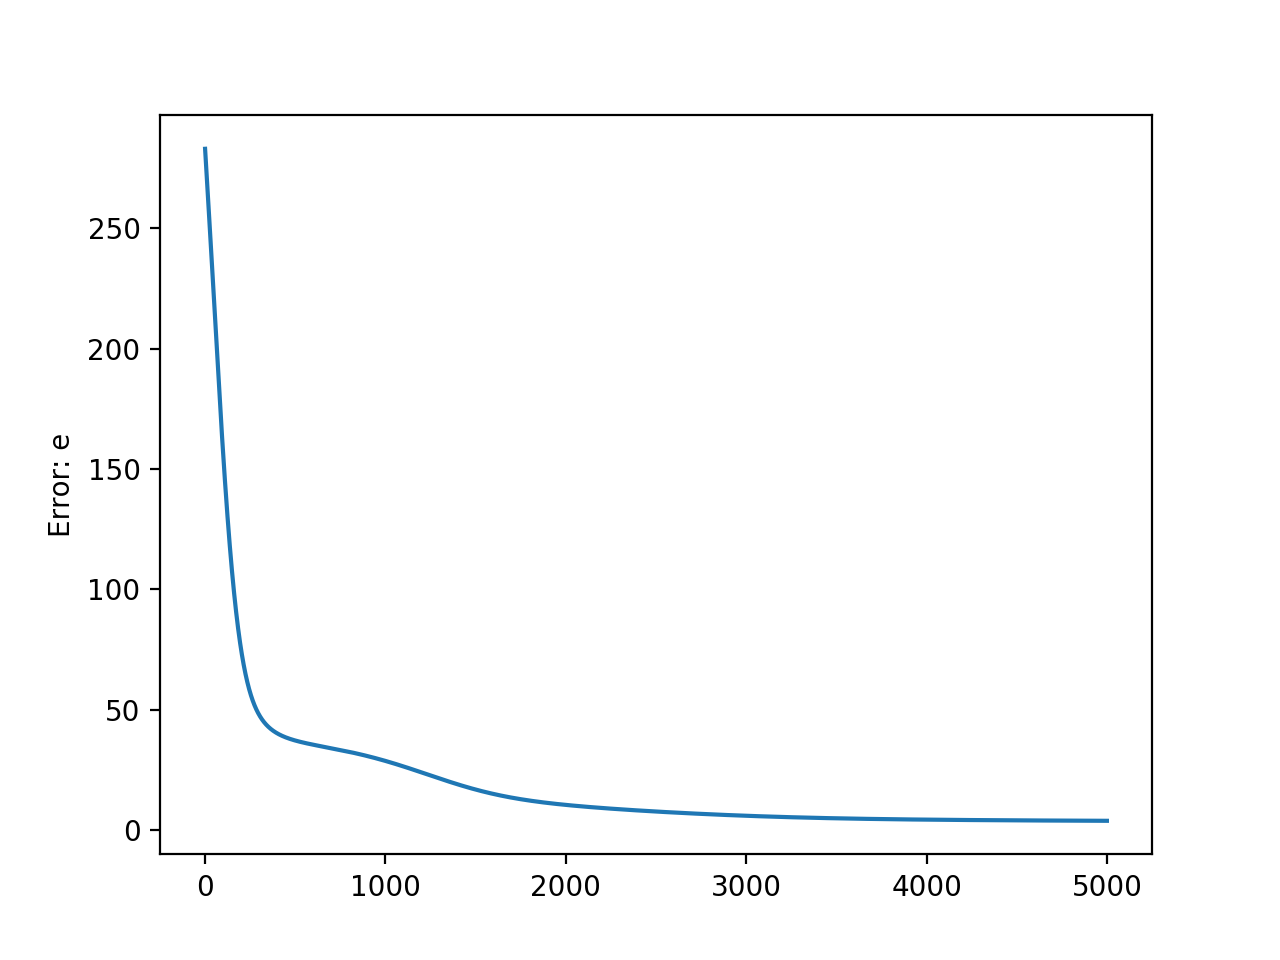
\includegraphics[scale=0.5]{Plot_Error}
	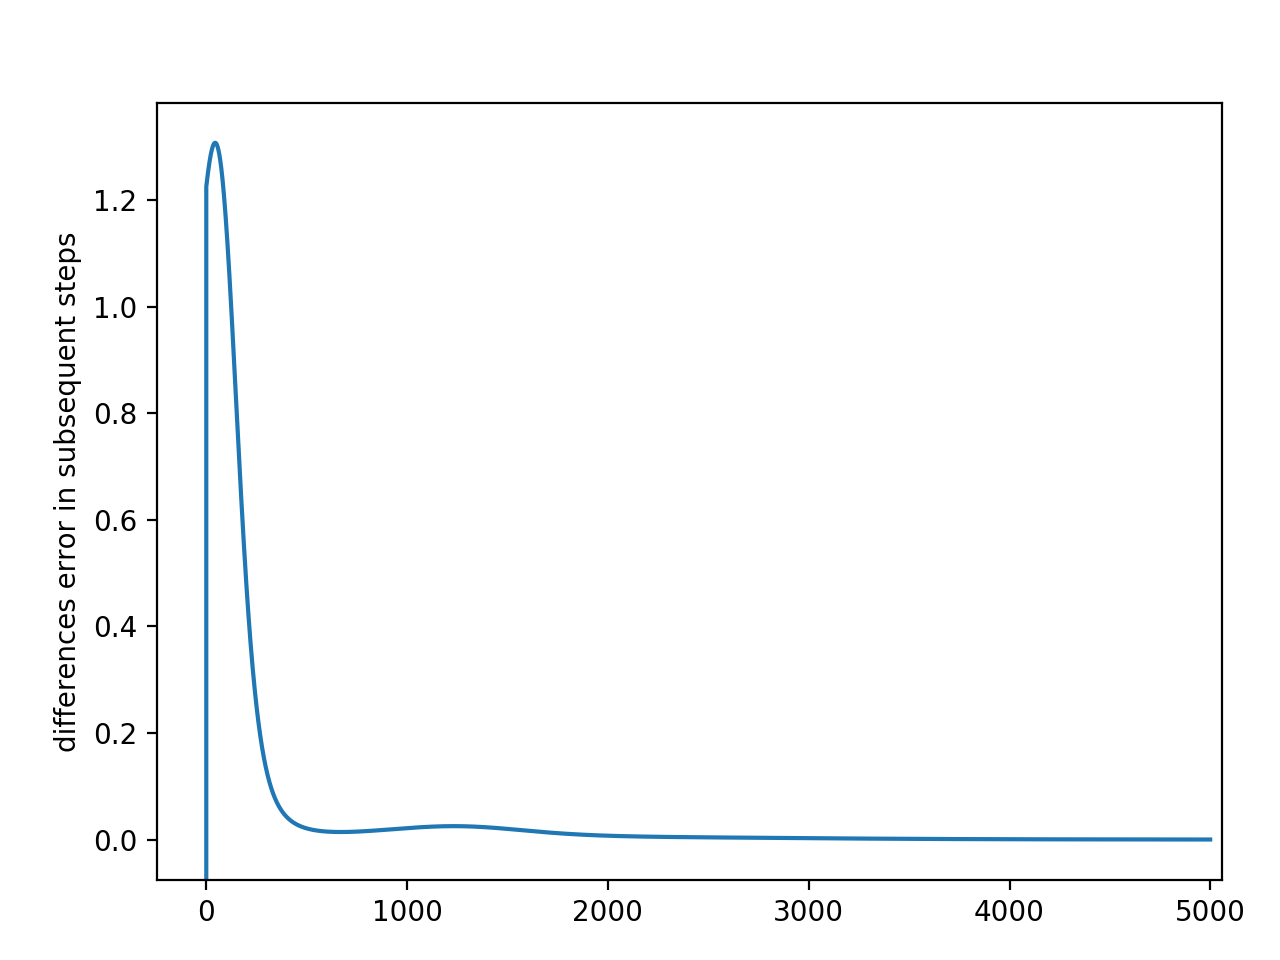
\includegraphics[scale=0.5]{DEISS_Zoomed}
	\\
	Note: More information in file: Error\_Values.txt
	
	\item [c)] Bonus, 3 points: In this code the learning rate "alpha" is a constant (alpha = 0.0002). How could you change the code to speed up the convergence? Explain your idea and implement your solution.
	There are several aproaches to this problem:
		\begin{itemize}
		\item 1. One is to set alpha to a value and divide it by the number of data (alpha/N)
		\item 2. Another one is the "Bold Driver" method where the alpha is changed in every iteration. If the error decreases you have to increase the alpha learning rate. If the error value increases (because we jumped over a minima) then you go 1 iteration back and decrease the learning-rate alpha.
		\item 3. Another: where you start with a "big" alpha and decrease it in every iteration with a appropriate value
		
		My Idea is Option (2) implementation code:\\
		 look into: U5\_Ex5\_mod.py\\
		 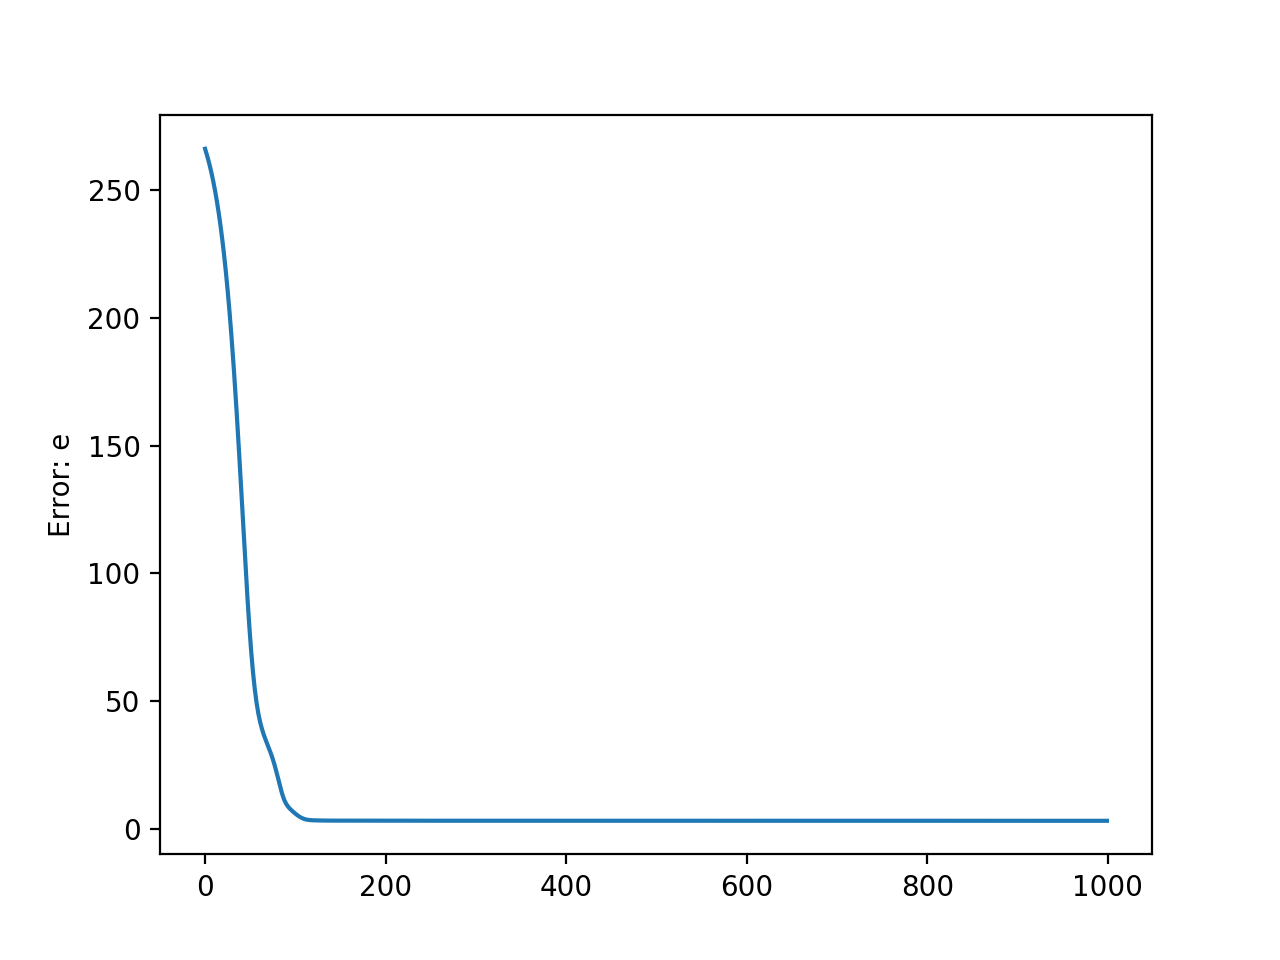
\includegraphics[scale=0.5]{Plot_Error_modAlpha}
		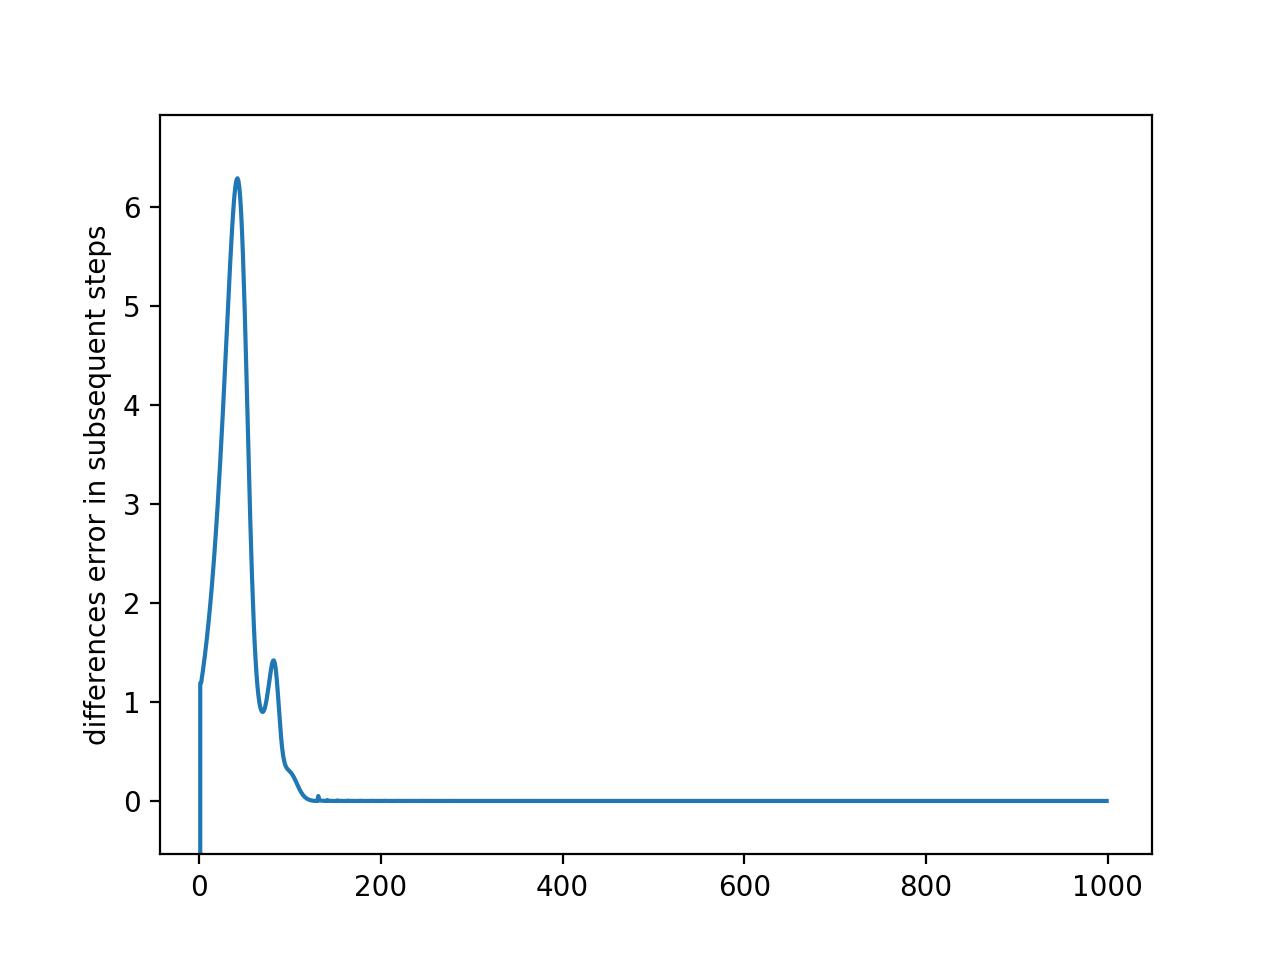
\includegraphics[scale=0.5]{DEISS_Zoomed_modAlpha}
		
		
		
	\end{itemize}
\end{itemize}
	
\end{document}
